\documentclass[11pt,a4paper]{article}
\usepackage[margin=1.1in]{geometry}
\usepackage{amsmath,amssymb,amsthm}
\usepackage{tikz}
\usepackage[hidelinks]{hyperref}
\urlstyle{same}

\newtheorem{lemma}{Lemma}
\newtheorem{theorem}{Theorem}
\theoremstyle{remark}
\newtheorem*{remark}{Remark}

\title{Pythagoras' theorem by counting lattice points}
\author{Tom Maciejewski\thanks{Independent researcher, New Jersey, USA. Email: \texttt{tommaciejewski4@gmail.com}}}
\date{November 2026}

\begin{document}
\maketitle

\begin{abstract}
For a right triangle with integer legs $a,b$, Pick's theorem measures the square
on the hypotenuse by counting the lattice points in it, and the count comes to
$a^2+b^2$. The idea is classroom folklore. We write the argument out in full,
extend it to all right triangles by a limit, and say what it really is: the
oldest dissection proof of the theorem, expressed in lattice points. We also
locate the geometry. The counts cannot see lengths at all; the Euclidean content
lies entirely in the fact that a square has the same area in every position.
\end{abstract}

\noindent
No theorem has been proved more often. Loomis's classic compilation
\cite{loomis} runs to 370 proofs, and the genre is still alive enough for the
\emph{Monthly} to have published new trigonometric proofs in 2024
\cite{jackson-johnson}. This note re-reads the oldest dissection proof through
Pick's theorem: the square on the hypotenuse is measured by counting the lattice
points in it.

The idea is close to a piece of classroom folklore. Generations of pupils have
drawn ``tilted squares'' on dotty paper and computed their areas by boxing and
subtracting corner triangles, discovering $x^2+y^2$ experimentally
\cite{nrich, picciotto}; and teachers have long noticed Pick's theorem standing
next to the activity. Chakerian and Kreith mention Pick's theorem as ``an
alternative way of finding the areas'' of tilted squares \cite{chakerian}, and
a GeoGebra applet counts the points of the hypotenuse square dynamically
\cite{mil}.

In 2021 a Mathematics Stack Exchange question \cite{mse} asked whether Pick's
theorem can prove Pythagoras' theorem. It treated only squares with $B=4$
boundary points, taking the interior count from pictures, which a commenter
called circular. Another comment reduced the problem to coprime legs and asked
for that count; the accepted answer proposed, without details, a general count
on a dissection figure; and a later comment objected that legs with irrational
ratio are out of reach unless patched by a limit, in which case Jordan area is
easier. We have not found the argument written out in full, although every
ingredient is standard. The purpose of this note is to write it out, to show
that it is the classical dissection in another language, and to say exactly
where the geometry enters.

\subsection*{The counting lemmas}

Throughout, the plane is the Euclidean plane of Hilbert's axioms, lengths are
real numbers, and coordinates only label a square grid; no distance formula is
used. Area is a positive function on polygons, additive, equal on congruent
polygons and $1$ on the unit square; its existence is classical
\cite[\S20]{hilbert}.

Let the right triangle have legs $a,b$ and hypotenuse $c$. Suppose first that
$a,b$ are positive integers, and let $d=\gcd(a,b)$. Place the triangle with its
right angle at the origin:
\[
C=(0,0),\qquad A=(0,b),\qquad B=(a,0).
\]
Rotating the vector $B-A=(a,-b)$ by a quarter turn gives $(b,a)$, so the square
erected on $AB$, on the side away from $C$, has vertices
\[
A=(0,b),\quad B=(a,0),\quad B+(b,a)=(a+b,a),\quad A+(b,a)=(b,a+b),
\]
all lattice points. (Its four sides are hypotenuses of triangles congruent to
$ABC$ by SAS, and its angles are right because the acute angles of $ABC$ add up
to a right angle.) Write $I_{\square}$ and $B_{\square}$ for the numbers of
lattice points interior to this square and on its boundary.

\begin{lemma}\label{lem:segment}
A segment between lattice points whose difference vector is $(x,y)\ne(0,0)$
contains exactly $\gcd(|x|,|y|)+1$ lattice points.
\end{lemma}

\begin{proof}
Let $g=\gcd(|x|,|y|)$. The points of the segment are $P+t(x,y)$ for
$0\le t\le 1$. If $t(x,y)$ is integral then $t$ is rational, since
$(x,y)\ne(0,0)$; writing $t=p/q$ in lowest terms forces $q\mid x$ and $q\mid y$,
hence $q\mid g$ and $t\in\{0,\tfrac1g,\dots,1\}$; conversely each $t=k/g$ gives
the lattice point $P+k\,(x/g,\,y/g)$.
\end{proof}

\begin{lemma}\label{lem:boundary}
$B_{\square}=4d$.
\end{lemma}

\begin{proof}
The four sides have difference vectors $(a,-b)$, $(b,a)$, $(-a,b)$, $(-b,-a)$,
each with coordinate gcd $d$. By Lemma~\ref{lem:segment} each side carries
$d+1$ lattice points; summing and correcting for the four double-counted
vertices, $B_{\square}=4(d+1)-4=4d$.
\end{proof}

\begin{lemma}\label{lem:triangle}
The triangle $ABC$ contains $I_{\triangle}=\tfrac12\bigl((a-1)(b-1)-(d-1)\bigr)$
interior lattice points.
\end{lemma}

\begin{proof}
The open rectangle $(0,a)\times(0,b)$ contains $(a-1)(b-1)$ lattice points, of
which, by Lemma~\ref{lem:segment}, exactly $d-1$ lie on the diagonal $AB$. The
half-turn $(x,y)\mapsto(a-x,\,b-y)$ about the rectangle's centre preserves the
lattice and the rectangle, maps the diagonal to itself, and swaps the two open
triangles; so the remaining $(a-1)(b-1)-(d-1)$ points split equally between
them.
\end{proof}

\subsection*{Pick's theorem, and why it may be used here}

\begin{lemma}[Pick \cite{pick}]\label{lem:pick}
A simple polygon with lattice-point vertices, containing $I$ lattice points in
its interior and $B$ on its boundary, has area $I+\tfrac12 B-1$.
\end{lemma}

Because this note uses Pick's theorem to \emph{prove} Pythagoras' theorem, it
matters that Pick's theorem can be proved without it; it can, and usually is.
The functional $F=I+\tfrac12B-1$ is additive when two polygons are glued along
a common boundary path (the $k$ interior points of the path move from boundary
to interior, and $F$ changes by $k-\tfrac12(k+1)-\tfrac12(k+1)+1=0$ across the
two pieces); area is additive too; and the two agree on axis-parallel
rectangles, then on right triangles with axis-parallel legs (halve a rectangle
and use the half-turn trick of Lemma~\ref{lem:triangle} on the diagonal), then
on arbitrary lattice triangles (box a triangle and subtract), then on all
lattice polygons (triangulate). Every step is bookkeeping with additivity of
area, its invariance under translations and half-turns, and the area $1$ of a
unit cell; no distance formula, no metric identity, and in particular no
Proposition I.47 enters. The additive route is written out by Picciotto
\cite{picciotto-pick}; Trainin \cite{trainin} gives another elementary proof.

\subsection*{The theorem, for integer legs}

\begin{lemma}\label{lem:square}
A square of side $s$, in any position, has area $s^2$.
\end{lemma}

\begin{proof}
By congruence we may take it axis-parallel. For rational $s$ it is tiled by
copies of a small square, and a real $s$ lies between rationals, area being
monotone.
\end{proof}

\begin{theorem}\label{thm:integer}
If the legs $a,b$ are integers, then $c^2=a^2+b^2$.
\end{theorem}

\begin{proof}
Enclose the tilted square in the box $[0,a+b]^2$ (Figure~1). The box is tiled
by the square together with four copies of the triangle, one in each corner:
they are the images of $ABC$ under the powers of the lattice-preserving quarter
turn $(x,y)\mapsto(a+b-y,\,x)$, so each has $I_{\triangle}$ interior lattice
points. The four hypotenuses --- the sides of the square --- run through the
interior of the box, while the square's vertices lie on the box's boundary. The
$(a+b-1)^2$ interior lattice points of the box therefore split as
\[
(a+b-1)^2 \;=\; I_{\square} \;+\; 4\,I_{\triangle}
\;+\; \underbrace{4(d-1)}_{\text{interior points of the four shared edges}}.
\]
Substituting Lemma~\ref{lem:triangle} and simplifying,
\[
I_{\square} \;=\; (a+b-1)^2-2\bigl((a-1)(b-1)-(d-1)\bigr)-4(d-1)
\;=\; a^2+b^2+1-2d .
\]
Now Lemma~\ref{lem:pick} with Lemma~\ref{lem:boundary}:
\[
\operatorname{Area}(\square)\;=\;I_{\square}+\tfrac12B_{\square}-1
\;=\;\bigl(a^2+b^2+1-2d\bigr)+2d-1\;=\;a^2+b^2 .
\]
The square has side $c$, so by Lemma~\ref{lem:square} its area is $c^2$; hence
$c^2=a^2+b^2$. This is the one point where lengths meet the count. It rests on a
square having the same area in every position, which in coordinates is
equivalent to the theorem and so must come from the theory of area.
\end{proof}

\begin{figure}[ht]
\centering
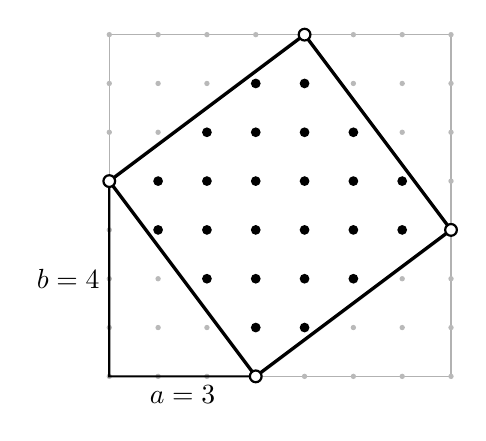
\begin{tikzpicture}[scale=0.62]
  \draw[gray!60] (0,0) rectangle (7,7);
  \foreach \x in {0,...,7} \foreach \y in {0,...,7}
    \fill[gray!55] (\x,\y) circle (0.055);
  \draw[thick] (0,0)--(3,0)--(0,4)--cycle;
  \node[below] at (1.5,0) {$a=3$};
  \node[left]  at (0,2)   {$b=4$};
  \draw[very thick] (0,4)--(3,0)--(7,3)--(4,7)--cycle;
  \foreach \p in {(1,3),(1,4),(2,2),(2,3),(2,4),(2,5),(3,1),(3,2),(3,3),(3,4),(3,5),(3,6),(4,1),(4,2),(4,3),(4,4),(4,5),(4,6),(5,2),(5,3),(5,4),(5,5),(6,3),(6,4)}
    \fill \p circle (0.10);
  \foreach \p in {(0,4),(3,0),(7,3),(4,7)}
    { \fill[white] \p circle (0.12); \draw[thick] \p circle (0.12); }
\end{tikzpicture}
\caption{The $3$--$4$--$5$ case: $d=1$, so the square's boundary carries
$B=4$ lattice points (circles) and its interior $I=24$ (solid);
Pick gives $24+\tfrac42-1=25=3^2+4^2$.}
\end{figure}

\subsection*{All right triangles}

\begin{theorem}\label{thm:general}
$c^2=a^2+b^2$ for every right triangle.
\end{theorem}

\begin{proof}
\emph{Rational legs} $a=p/q$, $b=r/q$: take $1/q$ as the unit of length. Every
length is then multiplied by $q$, so the legs are the integers $p,r$ and the
hypotenuse is $qc$. Theorem~\ref{thm:integer} holds for any unit, so
$(qc)^2=p^2+r^2$; divide by $q^2$.

\emph{Real legs}: choose positive rationals $a_n\to a$, $b_n\to b$, and place each
rational-legged triangle with its right angle at $C$, its legs along the rays
$CB$ and $CA$. Writing $A_n,B_n$ for its acute vertices and $c_n$ for its
hypotenuse, two applications of the triangle inequality give
\[
|c-c_n|\;\le\;|AA_n|+|BB_n|\;=\;|b-b_n|+|a-a_n|\;\longrightarrow\;0 ,
\]
so $c^2=\lim c_n^{\,2}=\lim\,(a_n^2+b_n^2)=a^2+b^2$.
\end{proof}

\begin{remark}
The objection in \cite{mse} is fair: Pick's theorem cannot see a triangle whose
legs have irrational ratio, the limit above is the patch, and area for real
sides, already used in Lemma~\ref{lem:square}, would be the shorter route. The
limit itself needs only the triangle inequality (Euclid I.20), which comes before
I.47 in the \emph{Elements}. The proof uses the parallel axiom (for the grid,
rectangles and quarter turn), SAS, real lengths with I.20, an area function with
Lemma~\ref{lem:square}, the gcd counts of
Lemmas~\ref{lem:segment}--\ref{lem:triangle}, and Pick's theorem. It uses no
distance formula, trigonometric identity or law of cosines.
\end{remark}

\subsection*{Discussion}

The reader will have recognised the $(a+b)\times(a+b)$ box: it is the figure of
the oldest dissection proofs (the \emph{Zhou Bi} diagram; Bh\=askara's figure is
its inner form). The argument is that dissection in another language. Since
$F=I+\tfrac12B-1$ is additive, with $F(\text{box})=(a+b)^2$ and
$F(\triangle)=ab/2$, the count is the identity
$(a+b)^2=\operatorname{Area}(\square)+2ab$ written in lattice points, and $d$
cancels because it already cancels inside each triangle. What is gained is a new
way of seeing the figure, not independence from it.

The counts cannot supply the Euclidean content. The shear
$(x,y)\mapsto(x+y,\,y)$ preserves the lattice, every count above and Pick's
formula, but not lengths or right angles. All of the geometry sits in
Lemma~\ref{lem:square}. Cameron \cite{cameron} gives the direct proofs from this
figure and makes the same point: what lies underneath them is that Euclidean
motions preserve area.

On priority: the ingredients of the argument are all standard, the classroom
observation that Pick's formula ``sees'' the hypotenuse square goes back at least
to about 1996 \cite{chakerian} (see also \cite{mil}), and a partial attempt was
posted publicly in 2021 \cite{mse}. What we have not found written out is the
chain itself: the interior count obtained from the box partition rather than from
the theorem, the boundary count $4d$, Pick's theorem and a limit. Two articles
on the geoboard and the theorem \cite{ewbank, naraine} may overlap with it; we
have not been able to consult them. Given how often proofs of this theorem are
rediscovered, the author would be glad to be sent an earlier reference, and makes
no stronger claim than ``not found after a genuine search.''

\begin{thebibliography}{99}

\bibitem{loomis} E. S. Loomis, \emph{The Pythagorean Proposition}, 2nd edn.
(1940), reissued by the National Council of Teachers of Mathematics (1968).

\bibitem{jackson-johnson} N. Jackson and C. Johnson, Five or ten new proofs of
the Pythagorean theorem, \emph{Amer. Math. Monthly} \textbf{131} (2024)
no.~9, pp.~739--752. \url{https://doi.org/10.1080/00029890.2024.2370240}

\bibitem{nrich} NRICH (Millennium Mathematics Project, Cambridge), Tilted
squares, \url{https://nrich.maths.org/problems/tilted-squares} (accessed
November 2026).

\bibitem{picciotto} H. Picciotto, The Pythagorean geoboard (1997),
\url{https://www.mathed.page/geoboard/geoboard.html} (accessed November 2026).

\bibitem{chakerian} G. D. Chakerian and K. Kreith, The Pythagorean theorem
(c.~1996), \url{http://www.mathematicallycorrect.com/pythag.htm} (accessed
November 2026).

\bibitem{mil} Jerzy Mil, Twierdzenie Pitagorasa i wz\'or Picka, GeoGebra applet
(2012), \url{https://www.geogebra.org/m/DG3ZyDqY} (accessed November 2026).

\bibitem{mse} vengy, Moti et al., Trying to prove the Pythagorean theorem using
Picks theorem, Mathematics Stack Exchange (September--November 2021),
\url{https://math.stackexchange.com/q/4256828} (accessed November 2026).

\bibitem{hilbert} D. Hilbert, \emph{The Foundations of Geometry}, transl. E. J.
Townsend, Open Court (1902). \url{https://math.berkeley.edu/~wodzicki/160/Hilbert.pdf}

\bibitem{picciotto-pick} H. Picciotto, Proving Pick's formula,
\url{https://www.mathed.page/geometry-labs/pick/} (accessed November 2026).

\bibitem{trainin} J. Trainin, An elementary proof of Pick's theorem,
\emph{Math.\ Gaz.} \textbf{91} (2007) no.~522, pp.~536--540 (Note 91.70).
\url{https://doi.org/10.1017/S0025557200182270}

\bibitem{pick} G. Pick, Geometrisches zur Zahlenlehre,
\emph{Sitzungsberichte des deutschen naturwissenschaftlich-medicinischen
Vereines f\"ur B\"ohmen ``Lotos'' in Prag} (2) \textbf{19} (1899)
pp.~311--319.

\bibitem{cameron} P. J. Cameron, Three easy proofs of Pythagoras' theorem, blog
post (8 May 2026),
\url{https://cameroncounts.wordpress.com/2026/05/08/three-easy-proofs-of-pythagoras-theorem/}.

\bibitem{ewbank} W. A. Ewbank, If Pythagoras had a geoboard\ldots,
\emph{Math.\ Teacher} \textbf{66} (1973) no.~3, pp.~215--221.
\url{https://doi.org/10.5951/mt.66.3.0215}

\bibitem{naraine} B. Naraine, K. A. Dotseth, G. Kim and M. Moody, If Pythagoras
had a geoboard\ldots, \emph{Math.\ Teacher} \textbf{86} (1993) no.~2,
pp.~137--139. \url{https://doi.org/10.5951/mt.86.2.0137}

\end{thebibliography}

\end{document}
